\subsection{Seleção dos revestimentos}

A aplicação com uso de Accura Spray para ajuste de parâmetros é
realizado para avaliar as modificações de vazão de gases no ajuste da
chama de aspersão. Para cada configuração de mistura de gases é registrado a
velocidade e temperatura da partícula aspergida a fim de se obter o melhor
parâmetro de aspersão, melhorando o rendimento e as propriedades do
revestimento. Foram utilizados 5 parâmetros de aspersão com o material de
Carboneto de Tungstênio-Cobalto Cromo com tamanho de grão entre 11 microns e 45 microns
(WCCoCr). O parâmetro que forneceu revestimento com menor nível de porosidade
foi replicado para aspergir material com Carboneto de Tungstênio-Cobalto Cromo
com tamanho de grão entre 15 microns e 45 microns (WS11) e material com
Carboneto de Tungstênio-Niquel Cromo (WCNi). Para todos os materiais foram
realizados ensaios para avaliação de resistência à corrosão, além do material
em aço inoxidável AISI 410 sem revestimento.

A aspersão com uma pistola de coating do tipo DJ2700 forneceu a
melhor característica de chama com os seguintes parâmetros: vazão de 72 L/min a
100 Psi de Combustível; vazão de 260 L/min a 150 Psi de Oxigênio; vazão de 340
L/min a 100 Psi de Ar comprimido; taxa de alimentação de pó de 40 g/min;
distância de trabalho de 230 mm; ângulo de aspersão de $90\circ$; velocidade de
deslocamento da pistola de 500 mm/s; velocidade de chama medida de 700 m/s; e
temperatura de chama medida de $1780\circ$C via Accura Spray. Os testes
destrutivos em corpos de prova WCCoCr e WCNi são realizados nestas condições.

\subsubsection{Análise dos substratos à corrosão}
As técnicas empregadas no estudo de resistência a corrosão dos sistemas (aço
inox AISI 410 recoberto por HVOF por camadas a base de WC) são: registro do
potencial do circuito aberto (OCP); e curvas de polarização eletroquímica. 

O potencial de circuito aberto é uma das variáveis que pode indicar a
suscetibilidade à corrosão. Em geral, quanto menor esse valor, maior será à
corrosão do sistema em estudo. Há uma tendência de que o material corroa mais no
sistema que apresente potenciais mais baixos em relação ao que apresente
potenciais mais altos. O potencial de circuito aberto (OCP) é medido por 60
minutos e, em seguida, é realizado ensaio de polarização potenciodinâmica
por um potenciostato/galvanostato, e uma célula eletroquímica,
onde a qual é disposta em uma gaiola de Faraday para diminuir as interferências
elétro-magnéticas externas. Este OCP pode ser observado também nas curvas
de polarização quando a corrente tende a zero.

A curva de polarização eletroquímica é outra análise que permite avaliar o
comportamento à corrosão de um determinado sistema metal-meio. Nessa técnica,
pode-se modificar o potencial de repouso (potencial de circuito aberto) para
valores mais positivos de potencial acelerando o processo corrosivo. A taxa de
corrosão esperada será proporcional à densidade de corrente registrada. Esse
ensaio permite determinar o potencial de pite, o qual será o potencial onde se
observa um aumento brusco de corrente.

Para todos os ensaios foi utilizada uma célula convencional de três eletrodos,
com eletrodo de calomelano saturado (ECS) como eletrodo de referência e eletrodo
de platina como contra eletrodo. As medidas foram realizadas em solução aquosa
de 3,5\% de NaCl em peso, não agitada, naturalmente aerado e à temperatura
ambiente. O potencial de circuito aberto (OCP) foi monitorado durante a primeira
hora de imersão no eletrólito antes do ensaio de polarização. O intervalo de
varredura foi de -100 mV abaixo do potencial de circuito aberto até 300 mV acima
do OCP, com uma velocidade de varredura de 1 mV/s.

Na Fig.~\ref{fig:adequacao4}, (A) mostra as curvas de potencial de circuito
aberto das amostras que sofreram variações nos parâmetros de deposição, com o
intuito de diminuir a porosidade dos revestimentos. Em todos os sistemas são
observados uma redução nqo potencial de circuito aberto com o decorrer do tempo,
podendo indicar um aumento de agressividade da solução presente nas
irregularidades das camadas revestidas.
Não é possível observar diferenças significantes entre as curvas OCP, no
entanto, o sistema 4 apresentou potenciais mais ativos de corrosão comparado com
os demais sistemas, possivelmente pelo alto nível de porosidade presentes no
revestimento.

\begin{figure}
	\centering
	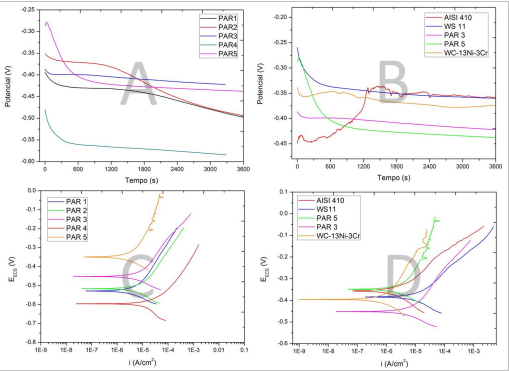
\includegraphics[width=1\columnwidth]{method/figs/adequacao/adequacao4.png}
    \caption{(A): Potencial de Circuito Aberto, com variação de parâmetros de
    aspersão térmica dos revestimentos de WC-10Co-4Cr com granulometria do pó
    11/45; (B) Potencial de Circuito Aberto de diferentes sistemas comparando
    com o substrato Jateado; (C) Ensaio de Polarização com variação de
    parâmetros dos revestimentos de WC-10Co-4Cr com granulometria do pó 11/45;
    (D) Ensaio de polarização dos diferentes sistemas comparando com o
    substrato jateado.}
    \label{fig:adequacao4}
\end{figure}

Para as curvas de OCP apresentadas na Fig.~\ref{fig:adequacao4} (B), foi
selecionado os dois revestimentos com menores porosidades nas medições
anteriores assim como o substrato, o WS 11 o qual foi utilizado pó com
granulometria diferente e o WCNi.

Conforme já comentado, os sistemas revestidos sofreram redução ao longo do tempo
pela provável modificação da solução no interior dos poros, ao contrário do
comportamento do substrato, que por ser maciço, não apresenta poros. Neste caso
observa-se um aumento do potencial de corrosão com o tempo, indicando redução no
processo corrosivo, possivelmente devido ao espessamento do filme protetor do
óxido de cromo.

Na Fig.~\ref{fig:adequacao4} (C), são apresentados os ensaios de polarização
eletroquímica da variação de alguns parâmetros operacionais. Nota-se que os
revestimentos com menores porosidades apresentam potencial de circuito aberto
(quando a curva tende a zero) mais elevado (menos negativos) indicando menor
taxa de corrosão. Além disso, à medida que a porosidade é reduzida, as curvas de
polarização tendem a se deslocar a esquerda, no sentido das menores correntes,
resultando em menores taxas de corrosão.

Na Fig.~\ref{fig:adequacao4} (D), são apresentadas as curvas de polarização dos
sistemas que tiveram menores porosidades e melhores desempenhos na
Fig.~\ref{fig:adequacao4} (C), o substrato de aço inoxidável AISI 410 jateado, a
amostra WS 11 utilizando um pó com granulometria de 15/45 e a amostra WCNi com
matriz de níquel. Analisando a Fig.~\ref{fig:adequacao4} (D), pode-se dizer
preliminarmente que os sistemas que apresentaram melhor desempenho frente a
corrosão, protegendo efetivamente o substrato, são os sistemas 5 e o WCNi. Esse
resultado é fruto de apenas uma técnica, necessitando de confirmação com outros
tipos de ensaios que considerem tempos mais longos de exposição das amostras ao
meio. Como, por exemplo, ensaio de imersão ou impedância eletroquímica.

Pode-se concluir que os teores de porosidade crescentes pioram o desempenho da
camada em proteger o substrato contra corrosão. Entre as camadas estudadas, as
que apresentaram efetiva proteção ao substrato foram os sistemas 5 e WCNi. A
presença de níquel no revestimento demonstra ser promissor em relação à proteção
do substrato à corrosão.

\subsubsection{Análise dos substratos à cavitação}
A metodologia dos ensaios de cavitação seguiu as recomendações da norma ASTM
G32, Standard Test Method for Cavitation Erosion Using Vibratory, que prevê duas
formas de realização dos testes: método direto e indireto. Um desenho
esquemático do equipamento utilizado para o teste via método direto pode ser
visualizado na Fig.\ref{fig:adequacao5}. O método indireto prevê que a amostra
permaneça imersa no bequer de água e com a face que deverá ser ensaiada de
frente para o sonotrodo a uma distância padrão. O sonotrodo é uma
dispositivo que está acoplado ao transdutor e vibra na frequência definida, induzindo um dano
por cavitação na superfície da amostra. Os parâmetros do ensaio estão
apresentados na Tabela~\ref{tab:param_hvof}. A frequência de vibração do
sonotrodo é ajustada através do módulo gerador de frequência utilizado pelo
laboratório do departamento de engenharia metalúrgica e de materiais da Universidade Federal de São Paulo
(USP).

\begin{figure}
	\centering
	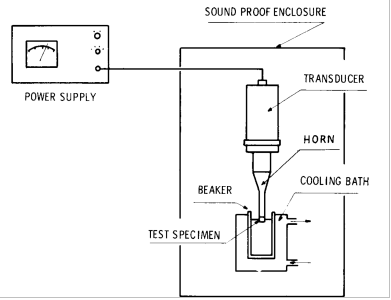
\includegraphics[width=1\columnwidth]{method/figs/adequacao/adequacao5.png}
    \caption{Desenho esquemático do ensaio de cavitação pelo método direto.
    Retirado da Norma ASTM G32.}
    \label{fig:adequacao5}
\end{figure}

\begin{table}[]
\centering
\caption{Parâmetros dos ensaios de cavitação conforme ASTM G32}
\label{tab:param_hvof}
\begin{tabular}{ll}
\hline
Parâmetro                                                 & Valor                                             \\ \hline
\multicolumn{1}{|l|}{Frequência de Vibração}              & \multicolumn{1}{l|}{20 kHz $\pm$ 0.5kHz}          \\ \hline
\multicolumn{1}{|l|}{Amplitude de Vibração}               & \multicolumn{1}{l|}{50 microns}                   \\ \hline
\multicolumn{1}{|l|}{Fluido de imersão}                   & \multicolumn{1}{l|}{Água destilada}               \\ \hline
\multicolumn{1}{|l|}{Temperatura da água}                 & \multicolumn{1}{l|}{$25^\circ$C $\pm$ $2^\circ$C} \\ \hline
\multicolumn{1}{|l|}{Profundidade de imersão}             & \multicolumn{1}{l|}{12 $\pm$ 4 mm}                \\ \hline
\multicolumn{1}{|l|}{Diâmetro do sonotrodo}               & \multicolumn{1}{l|}{15.9 $\pm$ 0.05 mm}           \\ \hline
\multicolumn{1}{|l|}{Distância entre amostra e sonotrodo} & \multicolumn{1}{l|}{0.5 mm}                       \\ \hline
\multicolumn{1}{|l|}{Tempo para cada ciclo de medição}    & \multicolumn{1}{l|}{20 min}                       \\ \hline
\multicolumn{1}{|l|}{Tempo total de ensaio por amostra}   & \multicolumn{1}{l|}{10h}                          \\ \hline
\end{tabular}
\end{table}

Os corpos de prova foram fabricados em material AISI 410 temperado e revestidos
de forma que a dureza final alcançada estivesse entre 34 e 37 HRC. As amostras
foram usinadas com geometria que atendesse à norma ASTM G32, ao encaixe no porta
amostra do equipamento de cavitação, e à facilidade de ser acoplada a um
dispositivo de metalização. Elas foram jateados até uma rugosidade mínima de 3.2
microns, foram instaladas na cabine de metalização do equipamento DJ2700 para
deposição dos recobrimentos. Para deixar a superfície mais adequada para
realização dos ensaios, todas as superfícies receberam leve polimento manual de
forma que todas as superfíces ficassem com rugosidade Ra normalizada abaixo de
2.5 microns.

A análise foi comparativa entre os dois revestimentos (WCCoCr e WCNiCr) em
relação ao material base AISI 410. Após as amostras terem sido preparadas  para
que ficassem com a mesma rugosidade superficial e próximo a 2.5 microns, foram
enviadas para a realização do ensaio, no qual o resultado será fornecido em
perda de massa para um mesmo tempo de ensaios nos três sistemas realizados.

Para avaliar a influência do acabamento superficial também foi realizado ensaio
em uma amostra de aço inox com polimento superior a fim de deixar a rugosidade
abaixo de Ra 0.32. O procedimento de ensaio consiste nas seguintes etapas:
\begin{itemize}
	\item Preparação superficial da amostra para ajuste da rugosidade através de
lixamento e polimento;
	\item Limpeza da amostra com alcool;
	\item Limpeza da amostra em ultrassom e acetona;
	\item Limpeza com álcool e secagem com ar quente;
	\item Pesagem inicial em balança de 5 dígitos;
	\item Fixação da amostra no dispositivo;
	\item Execução do ensaio por 20 min;
	\item Limpeza conforme itens b, c, d;
	\item Nova pesagem;
	\item Nova execução de ensaio por mais vinte minutos e repetição de todo o
procedimento até completar 10 horas de ensaio.
\end{itemize}

A realizaçao do estudo de cavitação utilizou os materiais do metal
base em aço Inoxidável AISI 410, além de amostras revestidas com materiais a
base de WC em matriz de Cobalto e cromo e a base de WC com matriz de Niquel e
Cromo. Para identificação das amostras durante condução dos testes, a seguinte
nomenclatura foi utilizada:

\begin{enumerate}
  \item WCNi: metal base em aço inioxidável, revestido com 0.2 mm de Carboneto  
  de Tungstênio em   matriz metálica de Niquel-Cromo pelo processo HVOF e sem
  acabamento supercial alcançando rugosidade de mínima de 2.2 microns.
  \item WCCoCr: metal base em aço inioxidável, revestido com 0.2 mm de
  Carboneto de Tungstênio em   matriz metálica de Cobaltol-Cromo pelo processo
  HVOF e sem acabamento supercial alcançando rugosidade mínima de 2.2 microns.
  \item 410: metal base em aço inioxidável, sem revestimento, com a superfície
  jateada e leve  acabamento supercial para produção de rugosidade mínima de
  2.2 microns.
  \item 410P: metal base em aço inioxidável, sem revestimento, com superfíce
  acabada através de lixamento progressivo desde lixa 80 até 600 para atingir
  rugosidade máxima de 0,4 microns.
\end{enumerate}
 
 Um resumo das características das amostras está apresentado na
 Tabela~\ref{tab:cav_hvof}.
 
 \begin{table}[]
\centering
\caption{Resumo das propriedades dos materiais utilizados para ensaios de Cavitação}
\label{tab:cav_hvof}
\begin{tabular}{lllllll}
\hline
Amostra                      & Metal base                    & \multicolumn{1}{c}{Revestimento}                                                        & \begin{tabular}[c]{@{}l@{}}Método \\ de aplicação\end{tabular} & \begin{tabular}[c]{@{}l@{}}Espessura \\ de camada (mm)\end{tabular} & \begin{tabular}[c]{@{}l@{}}Rugosidade Ra \\ ($\mu m)$\end{tabular} & \begin{tabular}[c]{@{}l@{}}Dureza superfície \\ (HV)\end{tabular} \\ \hline
\multicolumn{1}{|l|}{WCNi}   & \multicolumn{1}{l|}{AISI 410} & \multicolumn{1}{l|}{\begin{tabular}[c]{@{}l@{}}84\% WC\\ 13\% Ni\\ 3\% Cr\end{tabular}} & \multicolumn{1}{l|}{HVOF}                                      & \multicolumn{1}{l|}{0.180-0.210}                                    & \multicolumn{1}{l|}{Min. 2.2}                                      & \multicolumn{1}{l|}{1000-1300}                                    \\ \hline
\multicolumn{1}{|l|}{WCCoCr} & \multicolumn{1}{l|}{AISI 410} & \multicolumn{1}{l|}{\begin{tabular}[c]{@{}l@{}}86\%WC\\ 10\% Co\\ 4\% Cr\end{tabular}}  & \multicolumn{1}{l|}{HVOF}                                      & \multicolumn{1}{l|}{0.180-0.210}                                    & \multicolumn{1}{l|}{Min. 2.2}                                      & \multicolumn{1}{l|}{1100-1400}                                    \\ \hline
\multicolumn{1}{|l|}{410}    & \multicolumn{1}{l|}{AISI 410} & \multicolumn{1}{l|}{N/A}                                                                & \multicolumn{1}{l|}{N/A}                                       & \multicolumn{1}{l|}{N/A}                                            & \multicolumn{1}{l|}{Min. 2.2}                                      & \multicolumn{1}{l|}{350-400}                                      \\ \hline
\multicolumn{1}{|l|}{410P}   & \multicolumn{1}{l|}{AISI 410} & \multicolumn{1}{l|}{N/A}                                                                & \multicolumn{1}{l|}{N/A}                                       & \multicolumn{1}{l|}{N/A}                                            & \multicolumn{1}{l|}{Máx. 0.4}                                      & \multicolumn{1}{l|}{350-400}                                      \\ \hline
\end{tabular}
\end{table}

Os resultados comparativos entre as amostras WCNi, WCCoCr e 410 estão
apresentados na Tabela~\ref{tab:cav_hvof2}, e no gráfico do
Fig.~\ref{fig:adequacao6}. Os resultados comparativos entre as amostras 410 e
410P estão apresentadas na Tabela~\ref{tab:cav_hvof3} e no gráfico da
Fig.~\ref{fig:adequacao7}.

\begin{table}[]
\centering
\caption{Tabela com medições de massa e cálculo de perda de massa durante ensaio de cavitação.}
\label{tab:cav_hvof2}
\begin{tabular}{ccccccccccc}
\cline{1-3} \cline{5-7} \cline{9-11}
\multicolumn{3}{c}{WC10Co4Cr}                                                                           &                       & \multicolumn{3}{c}{WCNi}                                                                               &                       & \multicolumn{3}{c}{410}                                                                                \\ \cline{1-3} \cline{5-7} \cline{9-11} 
\multicolumn{1}{|l|}{Tempo (min)} & \multicolumn{1}{l|}{Peso (g)} & \multicolumn{1}{l|}{Perda de massa} & \multicolumn{1}{l|}{} & \multicolumn{1}{l|}{Tempo (min)} & \multicolumn{1}{l|}{Peso (g)} & \multicolumn{1}{l|}{Perda de massa} & \multicolumn{1}{l|}{} & \multicolumn{1}{l|}{Tempo (min)} & \multicolumn{1}{l|}{Peso (g)} & \multicolumn{1}{l|}{Perda de massa} \\ \cline{1-3} \cline{5-7} \cline{9-11} 
\multicolumn{1}{|c|}{0}           & \multicolumn{1}{c|}{54.40645} & \multicolumn{1}{c|}{0.00000}        & \multicolumn{1}{l|}{} & \multicolumn{1}{c|}{0}           & \multicolumn{1}{c|}{54.00434} & \multicolumn{1}{c|}{0.00000}        & \multicolumn{1}{l|}{} & \multicolumn{1}{c|}{0}           & \multicolumn{1}{c|}{52.30166} & \multicolumn{1}{c|}{0.00000}        \\ \cline{1-3} \cline{5-7} \cline{9-11} 
\multicolumn{1}{|c|}{20}          & \multicolumn{1}{c|}{54.40252} & \multicolumn{1}{c|}{0.00393}        & \multicolumn{1}{l|}{} & \multicolumn{1}{c|}{20}          & \multicolumn{1}{c|}{54.00177} & \multicolumn{1}{c|}{0.00257}        & \multicolumn{1}{l|}{} & \multicolumn{1}{c|}{20}          & \multicolumn{1}{c|}{52.29752} & \multicolumn{1}{c|}{0.00414}        \\ \cline{1-3} \cline{5-7} \cline{9-11} 
\multicolumn{1}{|c|}{40}          & \multicolumn{1}{c|}{54.40160} & \multicolumn{1}{c|}{0.00485}        & \multicolumn{1}{l|}{} & \multicolumn{1}{c|}{40}          & \multicolumn{1}{c|}{54.00105} & \multicolumn{1}{c|}{0.00329}        & \multicolumn{1}{l|}{} & \multicolumn{1}{c|}{40}          & \multicolumn{1}{c|}{52.29634} & \multicolumn{1}{c|}{0.00532}        \\ \cline{1-3} \cline{5-7} \cline{9-11} 
\multicolumn{1}{|c|}{60}          & \multicolumn{1}{c|}{54.40044} & \multicolumn{1}{c|}{0.00601}        & \multicolumn{1}{l|}{} & \multicolumn{1}{c|}{60}          & \multicolumn{1}{c|}{54.0033}  & \multicolumn{1}{c|}{0.00401}        & \multicolumn{1}{l|}{} & \multicolumn{1}{c|}{60}          & \multicolumn{1}{c|}{52.29533} & \multicolumn{1}{c|}{0.00633}        \\ \cline{1-3} \cline{5-7} \cline{9-11} 
\multicolumn{1}{|c|}{80}          & \multicolumn{1}{c|}{54.39953} & \multicolumn{1}{c|}{0.00692}        & \multicolumn{1}{l|}{} & \multicolumn{1}{c|}{80}          & \multicolumn{1}{c|}{53.99907} & \multicolumn{1}{c|}{0.00527}        & \multicolumn{1}{l|}{} & \multicolumn{1}{c|}{80}          & \multicolumn{1}{c|}{52.29442} & \multicolumn{1}{c|}{0.00724}        \\ \cline{1-3} \cline{5-7} \cline{9-11} 
\multicolumn{1}{|c|}{100}         & \multicolumn{1}{c|}{54.39884} & \multicolumn{1}{c|}{0.00761}        & \multicolumn{1}{c|}{} & \multicolumn{1}{c|}{100}         & \multicolumn{1}{c|}{53.99901} & \multicolumn{1}{c|}{0.00533}        & \multicolumn{1}{c|}{} & \multicolumn{1}{c|}{100}         & \multicolumn{1}{c|}{52.29349} & \multicolumn{1}{c|}{0.00817}        \\ \cline{1-3} \cline{5-7} \cline{9-11} 
\multicolumn{1}{|c|}{120}         & \multicolumn{1}{c|}{54,39797} & \multicolumn{1}{c|}{0,00848}        & \multicolumn{1}{c|}{} & \multicolumn{1}{c|}{120}         & \multicolumn{1}{c|}{53.99863} & \multicolumn{1}{c|}{0.00571}        & \multicolumn{1}{c|}{} & \multicolumn{1}{c|}{120}         & \multicolumn{1}{c|}{52.29254} & \multicolumn{1}{c|}{0.00912}        \\ \cline{1-3} \cline{5-7} \cline{9-11} 
\multicolumn{1}{|c|}{180}         & \multicolumn{1}{c|}{54.39565} & \multicolumn{1}{c|}{0,01080}        & \multicolumn{1}{c|}{} & \multicolumn{1}{c|}{180}         & \multicolumn{1}{c|}{53.99734} & \multicolumn{1}{c|}{0.00700}        & \multicolumn{1}{c|}{} & \multicolumn{1}{c|}{180}         & \multicolumn{1}{c|}{52.28958} & \multicolumn{1}{c|}{0.01208}        \\ \cline{1-3} \cline{5-7} \cline{9-11} 
\multicolumn{1}{|c|}{240}         & \multicolumn{1}{c|}{54.39387} & \multicolumn{1}{c|}{0.01258}        & \multicolumn{1}{c|}{} & \multicolumn{1}{c|}{240}         & \multicolumn{1}{c|}{53.99610} & \multicolumn{1}{c|}{0.00824}        & \multicolumn{1}{c|}{} & \multicolumn{1}{c|}{240}         & \multicolumn{1}{c|}{52.28675} & \multicolumn{1}{c|}{0.01491}        \\ \cline{1-3} \cline{5-7} \cline{9-11} 
\multicolumn{1}{|c|}{300}         & \multicolumn{1}{c|}{54.39170} & \multicolumn{1}{c|}{0.01475}        & \multicolumn{1}{c|}{} & \multicolumn{1}{c|}{300}         & \multicolumn{1}{c|}{53.99503} & \multicolumn{1}{c|}{0.00931}        & \multicolumn{1}{c|}{} & \multicolumn{1}{c|}{300}         & \multicolumn{1}{c|}{52.28368} & \multicolumn{1}{c|}{0.01798}        \\ \cline{1-3} \cline{5-7} \cline{9-11} 
\multicolumn{1}{|c|}{360}         & \multicolumn{1}{c|}{54.39063} & \multicolumn{1}{c|}{0.01582}        & \multicolumn{1}{c|}{} & \multicolumn{1}{c|}{360}         & \multicolumn{1}{c|}{53.99404} & \multicolumn{1}{c|}{0.01030}        & \multicolumn{1}{c|}{} & \multicolumn{1}{c|}{360}         & \multicolumn{1}{c|}{52.28070} & \multicolumn{1}{c|}{0.02096}        \\ \cline{1-3} \cline{5-7} \cline{9-11} 
\multicolumn{1}{|c|}{420}         & \multicolumn{1}{c|}{54.38997} & \multicolumn{1}{c|}{0.01648}        & \multicolumn{1}{c|}{} & \multicolumn{1}{c|}{420}         & \multicolumn{1}{c|}{53.99263} & \multicolumn{1}{c|}{0.01171}        & \multicolumn{1}{c|}{} & \multicolumn{1}{c|}{420}         & \multicolumn{1}{c|}{52.27706} & \multicolumn{1}{c|}{0.02460}        \\ \cline{1-3} \cline{5-7} \cline{9-11} 
\multicolumn{1}{|c|}{480}         & \multicolumn{1}{c|}{54.38880} & \multicolumn{1}{c|}{0.01765}        & \multicolumn{1}{c|}{} & \multicolumn{1}{c|}{480}         & \multicolumn{1}{c|}{53.99150} & \multicolumn{1}{c|}{0.01284}        & \multicolumn{1}{c|}{} & \multicolumn{1}{c|}{480}         & \multicolumn{1}{c|}{52.27485} & \multicolumn{1}{c|}{0.02681}        \\ \cline{1-3} \cline{5-7} \cline{9-11} 
\multicolumn{1}{|c|}{540}         & \multicolumn{1}{c|}{54.38660} & \multicolumn{1}{c|}{0.01985}        & \multicolumn{1}{c|}{} & \multicolumn{1}{c|}{540}         & \multicolumn{1}{c|}{53.99010} & \multicolumn{1}{c|}{0.01424}        & \multicolumn{1}{c|}{} & \multicolumn{1}{c|}{540}         & \multicolumn{1}{c|}{52.27178} & \multicolumn{1}{c|}{0.02988}        \\ \cline{1-3} \cline{5-7} \cline{9-11} 
\multicolumn{1}{|c|}{600}         & \multicolumn{1}{c|}{54.38465} & \multicolumn{1}{c|}{0.02180}        & \multicolumn{1}{c|}{} & \multicolumn{1}{c|}{600}         & \multicolumn{1}{c|}{53.98912} & \multicolumn{1}{c|}{0.01522}        & \multicolumn{1}{c|}{} & \multicolumn{1}{c|}{600}         & \multicolumn{1}{c|}{52.26859} & \multicolumn{1}{c|}{0.03307}        \\ \cline{1-3} \cline{5-7} \cline{9-11} 
\end{tabular}
\end{table}

\begin{figure}
	\centering
	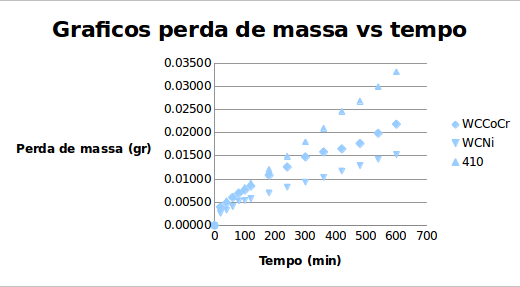
\includegraphics[width=1\columnwidth]{method/figs/adequacao/adequacao6.png}
    \caption{Resultados comparativos entre as amoostras de materiais distintos.}
    \label{fig:adequacao6}
\end{figure}

\begin{table}[]
\centering
\caption{Medições de perda de massa durante ensaio de cavitação das amostras 410P.}
\label{tab:cav_hvof3}
\begin{tabular}{ccccccc}
\cline{1-3} \cline{5-7}
\multicolumn{3}{c}{410 (Ra 2.2)}                                                                        &                       & \multicolumn{3}{c}{410P (Ra 0.4)}                                                                      \\ \cline{1-3} \cline{5-7} 
\multicolumn{1}{|l|}{Tempo (min)} & \multicolumn{1}{l|}{Peso (g)} & \multicolumn{1}{l|}{Perda de massa} & \multicolumn{1}{l|}{} & \multicolumn{1}{l|}{Tempo (min)} & \multicolumn{1}{l|}{Peso (g)} & \multicolumn{1}{l|}{Perda de massa} \\ \cline{1-3} \cline{5-7} 
\multicolumn{1}{|c|}{0}           & \multicolumn{1}{c|}{52,30166} & \multicolumn{1}{c|}{0,00000}        & \multicolumn{1}{l|}{} & \multicolumn{1}{c|}{0}           & \multicolumn{1}{c|}{52,15546} & \multicolumn{1}{c|}{0.00000}        \\ \cline{1-3} \cline{5-7} 
\multicolumn{1}{|c|}{20}          & \multicolumn{1}{c|}{52,29752} & \multicolumn{1}{c|}{0,00414}        & \multicolumn{1}{l|}{} & \multicolumn{1}{c|}{20}          & \multicolumn{1}{c|}{52,15495} & \multicolumn{1}{c|}{0,00051}        \\ \cline{1-3} \cline{5-7} 
\multicolumn{1}{|c|}{40}          & \multicolumn{1}{c|}{52,29634} & \multicolumn{1}{c|}{0,00532}        & \multicolumn{1}{l|}{} & \multicolumn{1}{c|}{40}          & \multicolumn{1}{c|}{52,15457} & \multicolumn{1}{c|}{0,00089}        \\ \cline{1-3} \cline{5-7} 
\multicolumn{1}{|c|}{60}          & \multicolumn{1}{c|}{52,29533} & \multicolumn{1}{c|}{0,00633}        & \multicolumn{1}{l|}{} & \multicolumn{1}{c|}{60}          & \multicolumn{1}{c|}{}         & \multicolumn{1}{c|}{}               \\ \cline{1-3} \cline{5-7} 
\multicolumn{1}{|c|}{80}          & \multicolumn{1}{c|}{52,29442} & \multicolumn{1}{c|}{0,00724}        & \multicolumn{1}{l|}{} & \multicolumn{1}{c|}{80}          & \multicolumn{1}{c|}{}         & \multicolumn{1}{c|}{}               \\ \cline{1-3} \cline{5-7} 
\multicolumn{1}{|c|}{100}         & \multicolumn{1}{c|}{52,29349} & \multicolumn{1}{c|}{0,00817}        & \multicolumn{1}{c|}{} & \multicolumn{1}{c|}{100}         & \multicolumn{1}{c|}{}         & \multicolumn{1}{c|}{}               \\ \cline{1-3} \cline{5-7} 
\multicolumn{1}{|c|}{120}         & \multicolumn{1}{c|}{52,29254} & \multicolumn{1}{c|}{0,00912}        & \multicolumn{1}{c|}{} & \multicolumn{1}{c|}{120}         & \multicolumn{1}{c|}{}         & \multicolumn{1}{c|}{}               \\ \cline{1-3} \cline{5-7} 
\multicolumn{1}{|c|}{180}         & \multicolumn{1}{c|}{52,28958} & \multicolumn{1}{c|}{0,01208}        & \multicolumn{1}{c|}{} & \multicolumn{1}{c|}{180}         & \multicolumn{1}{c|}{52,15273} & \multicolumn{1}{c|}{0,00273}        \\ \cline{1-3} \cline{5-7} 
\multicolumn{1}{|c|}{240}         & \multicolumn{1}{c|}{52,28675} & \multicolumn{1}{c|}{0,01491}        & \multicolumn{1}{c|}{} & \multicolumn{1}{c|}{}            & \multicolumn{1}{c|}{}         & \multicolumn{1}{c|}{}               \\ \cline{1-3} \cline{5-7} 
\multicolumn{1}{|c|}{300}         & \multicolumn{1}{c|}{52,28368} & \multicolumn{1}{c|}{0,01798}        & \multicolumn{1}{c|}{} & \multicolumn{1}{c|}{}            & \multicolumn{1}{c|}{}         & \multicolumn{1}{c|}{}               \\ \cline{1-3} \cline{5-7} 
\multicolumn{1}{|c|}{360}         & \multicolumn{1}{c|}{52,28070} & \multicolumn{1}{c|}{0,02096}        & \multicolumn{1}{c|}{} & \multicolumn{1}{c|}{}            & \multicolumn{1}{c|}{}         & \multicolumn{1}{c|}{}               \\ \cline{1-3} \cline{5-7} 
\multicolumn{1}{|c|}{420}         & \multicolumn{1}{c|}{52,27706} & \multicolumn{1}{c|}{0,02460}        & \multicolumn{1}{c|}{} & \multicolumn{1}{c|}{}            & \multicolumn{1}{c|}{}         & \multicolumn{1}{c|}{}               \\ \cline{1-3} \cline{5-7} 
\multicolumn{1}{|c|}{480}         & \multicolumn{1}{c|}{52,27485} & \multicolumn{1}{c|}{0,02681}        & \multicolumn{1}{c|}{} & \multicolumn{1}{c|}{}            & \multicolumn{1}{c|}{}         & \multicolumn{1}{c|}{}               \\ \cline{1-3} \cline{5-7} 
\multicolumn{1}{|c|}{540}         & \multicolumn{1}{c|}{52,27178} & \multicolumn{1}{c|}{0,02988}        & \multicolumn{1}{c|}{} & \multicolumn{1}{c|}{}            & \multicolumn{1}{c|}{}         & \multicolumn{1}{c|}{}               \\ \cline{1-3} \cline{5-7} 
\multicolumn{1}{|c|}{600}         & \multicolumn{1}{c|}{52,26859} & \multicolumn{1}{c|}{0,03307}        & \multicolumn{1}{c|}{} & \multicolumn{1}{c|}{}            & \multicolumn{1}{c|}{}         & \multicolumn{1}{c|}{}               \\ \cline{1-3} \cline{5-7} 
\end{tabular}
\end{table}
 
\begin{figure}
	\centering
	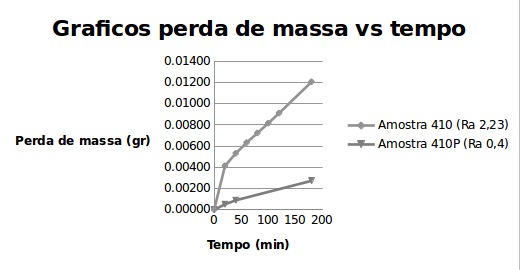
\includegraphics[width=1\columnwidth]{method/figs/adequacao/adequacao7.png}
    \caption{Influência do acabamento na taxa de desgaste por cavitação.}
    \label{fig:adequacao7}
\end{figure}

Pode-se concluir que ambos os revestimentos melhoram a resistência à cavitação
da superfície, tendo o revestimento WCNi a base de Carboneto de Tungstênio em
matriz de Niquel-Cromo rendimento aproximadamente 50\% superior ao revestimento
WCCoCr.

Após a entrega dos resultados comparativos entre as amostras com e sem
revestimento, foi realizada uma visita ao laboratório responsável pela execução
dos testes. Durante essa visita foram realizadas as seguintes atividades:

\begin{enumerate}
  \item Verificação da metodologia utilizada e dos parâmetros utilizados nos
  ensaios;
  \item Discussão técnica dos resultados;
  \item Preparação de amostras e realização de teste para verificação do efeito
  de rugosidade no desgaste por cavitação;
  \item Caracterização superficial com lupa de baixo aumento; 
\end{enumerate}

Foi realizada a análise dos resultados juntamente com os pesquisadores do
departamento de engenharia metalúrgica e de materiais da Universidade Federal de São Paulo 
realizadas com a análise de artigos técnicos referentes ao assunto de desgaste
por cavitação. Primeiramente os resultados encontrados foram comparados com os
resultados no artigo \cite{santa2009slurry}. Neste, o autor também verificou
aumento na resistência à cavitação das superfícies qa partir da aplicação de
revestimentos aspergidos termicamente.

A norma estebelece que a superfície antes do ensaios seja acabada até a lixa com
granulometria 600, o que não foi realizado por opção devido à tentativa de
reproduzir o acabamento o mais próximo da situação atual dos revestimentos das
pás, que entram em operação com uma rugosidade de material como aspergido, ou
seja sem nenhum acabamento posterior ao resvetimento. Nesse sentido a tese de
doutorado \cite{xiaojun2002effect} foi analisada e optou-se por realizar o
procedimento de acabamento de uma amostra em AISI 410 através de lixamentos
subsequentes até que a superfície ficasse com rugosidade abaixo de 0.4 $\mu$mRa
e então chamando essa amostra de 410P e realizando o ensaio seguindo o mesmo
procedimento já descrito anteriormento porém em intervalos maiores e menor tempo
total de ensaio, para verificar a tendência da curva de desgaste. Os resultados
comparativos podem ser analizados na Tabela~\ref{tab:cav_hvof3} e gráfico da
Fig.~\ref{fig:adequacao7}. Percebe-se que o acabamento exerce influência na taxa
de desgaste por cavitação, podendo ser um importante fator para retardar o dano
na pás com revestimento.

A caracterização da superfície em lupa de baixo aumento (8x) foi realizada a fim
de se observar trincas no revestimento após 10 h de ensaio. As imagens estão
apresentadas na Fig.~\ref{fig:adequacao8}.

\begin{figure}
	\centering
	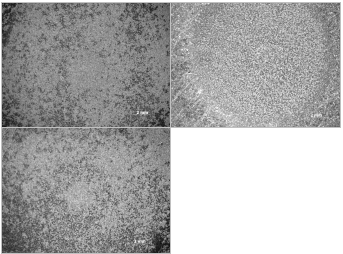
\includegraphics[width=1\columnwidth]{method/figs/adequacao/adequacao8.png}
    \caption{Superficies degastadas analisadas em Lupa com aumento de 8x após ensaios de cavitação. A) WCCoCr. B) AISI410. C)WCNi.}
    \label{fig:adequacao8}
\end{figure}